\documentclass[border=2mm]{standalone}
\usepackage{pgfplots}
\usepgfplotslibrary{groupplots}
\pgfplotsset{compat=1.18}
\definecolor{BCred}{rgb}{0.7, 0.11, 0.11}
\pgfplotsset{every axis/.append style={
  width=7.5cm, height=7.5cm, scale only axis,
  ticklabel style={font=\scriptsize, /pgf/number format/fixed, /pgf/number format/precision=2},
  yticklabel style={text width=10mm, align=right},
  ylabel style={text width=10mm, align=center},
  label style={font=\small},
  title style={font=\small},
  legend style={draw=none, font=\footnotesize}}}
\begin{document}
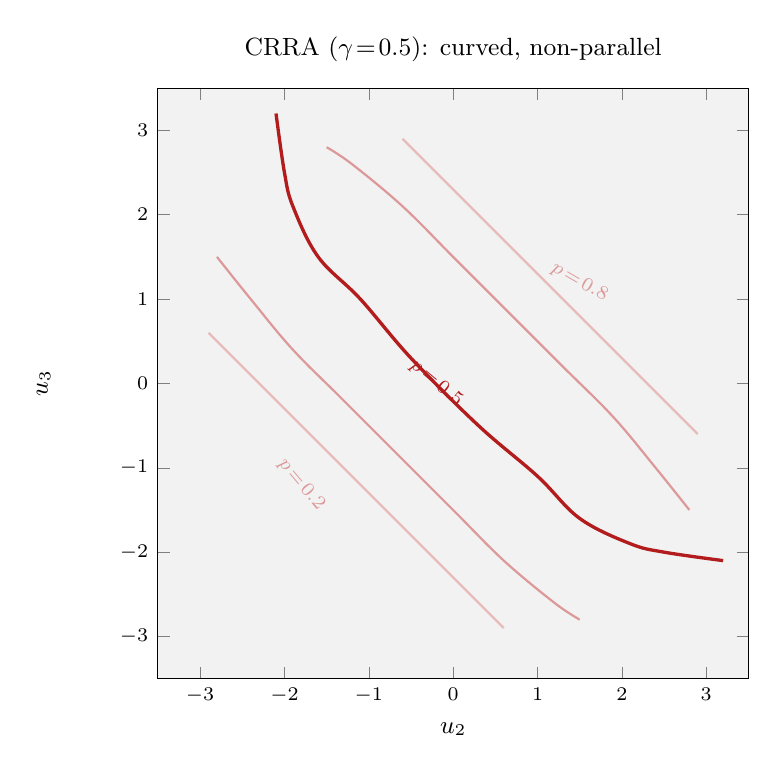
\begin{tikzpicture}
\begin{groupplot}[group style={group size=1 by 1}]
\nextgroupplot[
  xmin=-3.5, xmax=3.5, ymin=-3.5, ymax=3.5,
  xlabel={$u_2$}, ylabel={$u_3$},
  axis equal image,
  title={CRRA ($\gamma\!=\!0.5$): curved, non-parallel},
  axis background/.style={fill=black!5}]
% p=0.2 (projected, smooth curve)
\addplot[thick,color=BCred!30,smooth,tension=0.6] coordinates {
  (-2.9,0.6)(-2.5,0.2)(-2.0,-0.3)(-1.4,-0.9)(-0.8,-1.5)
  (-0.2,-2.1)(0.3,-2.6)(0.6,-2.9)};
% p=0.3 (projected)
\addplot[thick,color=BCred!45,smooth,tension=0.6] coordinates {
  (-2.8,1.5)(-2.4,1.0)(-1.9,0.4)(-1.3,-0.2)(-0.6,-0.9)
  (0.0,-1.5)(0.6,-2.1)(1.2,-2.6)(1.5,-2.8)};
% p=0.5 (from solver REE data, smoothed key points)
\addplot[very thick,color=BCred,smooth,tension=0.6] coordinates {
  (-2.1,3.2)(-2.0,2.5)(-1.9,2.1)(-1.6,1.5)(-1.1,1.0)
  (-0.5,0.3)(0.3,-0.5)(1.0,-1.1)(1.5,-1.6)(2.1,-1.9)
  (2.5,-2.0)(3.2,-2.1)};
% p=0.7 (projected)
\addplot[thick,color=BCred!45,smooth,tension=0.6] coordinates {
  (-1.5,2.8)(-1.2,2.6)(-0.6,2.1)(0.0,1.5)(0.6,0.9)
  (1.3,0.2)(1.9,-0.4)(2.4,-1.0)(2.8,-1.5)};
% p=0.8 (projected)
\addplot[thick,color=BCred!30,smooth,tension=0.6] coordinates {
  (-0.6,2.9)(-0.3,2.6)(0.2,2.1)(0.8,1.5)
  (1.4,0.9)(2.0,0.3)(2.5,-0.2)(2.9,-0.6)};
% Labels
\node[font=\scriptsize,color=BCred!45,rotate=-50] at (axis cs:-1.8,-1.2) {$p\!=\!0.2$};
\node[font=\scriptsize,color=BCred,rotate=-40] at (axis cs:-0.2,0.0) {$p\!=\!0.5$};
\node[font=\scriptsize,color=BCred!45,rotate=-30] at (axis cs:1.5,1.2) {$p\!=\!0.8$};
\end{groupplot}
\end{tikzpicture}
\end{document}
